\documentclass[]{article}
\usepackage{lmodern}
\usepackage{amssymb,amsmath}
\usepackage{ifxetex,ifluatex}
\usepackage{fixltx2e} % provides \textsubscript
\ifnum 0\ifxetex 1\fi\ifluatex 1\fi=0 % if pdftex
  \usepackage[T1]{fontenc}
  \usepackage[utf8]{inputenc}
\else % if luatex or xelatex
  \ifxetex
    \usepackage{mathspec}
  \else
    \usepackage{fontspec}
  \fi
  \defaultfontfeatures{Ligatures=TeX,Scale=MatchLowercase}
\fi
% use upquote if available, for straight quotes in verbatim environments
\IfFileExists{upquote.sty}{\usepackage{upquote}}{}
% use microtype if available
\IfFileExists{microtype.sty}{%
\usepackage{microtype}
\UseMicrotypeSet[protrusion]{basicmath} % disable protrusion for tt fonts
}{}
\usepackage[margin=1in]{geometry}
\usepackage{hyperref}
\hypersetup{unicode=true,
            pdftitle={Assignment-3},
            pdfauthor={Syed Muhammad Adeel Ibrahim},
            pdfborder={0 0 0},
            breaklinks=true}
\urlstyle{same}  % don't use monospace font for urls
\usepackage{color}
\usepackage{fancyvrb}
\newcommand{\VerbBar}{|}
\newcommand{\VERB}{\Verb[commandchars=\\\{\}]}
\DefineVerbatimEnvironment{Highlighting}{Verbatim}{commandchars=\\\{\}}
% Add ',fontsize=\small' for more characters per line
\usepackage{framed}
\definecolor{shadecolor}{RGB}{248,248,248}
\newenvironment{Shaded}{\begin{snugshade}}{\end{snugshade}}
\newcommand{\KeywordTok}[1]{\textcolor[rgb]{0.13,0.29,0.53}{\textbf{#1}}}
\newcommand{\DataTypeTok}[1]{\textcolor[rgb]{0.13,0.29,0.53}{#1}}
\newcommand{\DecValTok}[1]{\textcolor[rgb]{0.00,0.00,0.81}{#1}}
\newcommand{\BaseNTok}[1]{\textcolor[rgb]{0.00,0.00,0.81}{#1}}
\newcommand{\FloatTok}[1]{\textcolor[rgb]{0.00,0.00,0.81}{#1}}
\newcommand{\ConstantTok}[1]{\textcolor[rgb]{0.00,0.00,0.00}{#1}}
\newcommand{\CharTok}[1]{\textcolor[rgb]{0.31,0.60,0.02}{#1}}
\newcommand{\SpecialCharTok}[1]{\textcolor[rgb]{0.00,0.00,0.00}{#1}}
\newcommand{\StringTok}[1]{\textcolor[rgb]{0.31,0.60,0.02}{#1}}
\newcommand{\VerbatimStringTok}[1]{\textcolor[rgb]{0.31,0.60,0.02}{#1}}
\newcommand{\SpecialStringTok}[1]{\textcolor[rgb]{0.31,0.60,0.02}{#1}}
\newcommand{\ImportTok}[1]{#1}
\newcommand{\CommentTok}[1]{\textcolor[rgb]{0.56,0.35,0.01}{\textit{#1}}}
\newcommand{\DocumentationTok}[1]{\textcolor[rgb]{0.56,0.35,0.01}{\textbf{\textit{#1}}}}
\newcommand{\AnnotationTok}[1]{\textcolor[rgb]{0.56,0.35,0.01}{\textbf{\textit{#1}}}}
\newcommand{\CommentVarTok}[1]{\textcolor[rgb]{0.56,0.35,0.01}{\textbf{\textit{#1}}}}
\newcommand{\OtherTok}[1]{\textcolor[rgb]{0.56,0.35,0.01}{#1}}
\newcommand{\FunctionTok}[1]{\textcolor[rgb]{0.00,0.00,0.00}{#1}}
\newcommand{\VariableTok}[1]{\textcolor[rgb]{0.00,0.00,0.00}{#1}}
\newcommand{\ControlFlowTok}[1]{\textcolor[rgb]{0.13,0.29,0.53}{\textbf{#1}}}
\newcommand{\OperatorTok}[1]{\textcolor[rgb]{0.81,0.36,0.00}{\textbf{#1}}}
\newcommand{\BuiltInTok}[1]{#1}
\newcommand{\ExtensionTok}[1]{#1}
\newcommand{\PreprocessorTok}[1]{\textcolor[rgb]{0.56,0.35,0.01}{\textit{#1}}}
\newcommand{\AttributeTok}[1]{\textcolor[rgb]{0.77,0.63,0.00}{#1}}
\newcommand{\RegionMarkerTok}[1]{#1}
\newcommand{\InformationTok}[1]{\textcolor[rgb]{0.56,0.35,0.01}{\textbf{\textit{#1}}}}
\newcommand{\WarningTok}[1]{\textcolor[rgb]{0.56,0.35,0.01}{\textbf{\textit{#1}}}}
\newcommand{\AlertTok}[1]{\textcolor[rgb]{0.94,0.16,0.16}{#1}}
\newcommand{\ErrorTok}[1]{\textcolor[rgb]{0.64,0.00,0.00}{\textbf{#1}}}
\newcommand{\NormalTok}[1]{#1}
\usepackage{graphicx,grffile}
\makeatletter
\def\maxwidth{\ifdim\Gin@nat@width>\linewidth\linewidth\else\Gin@nat@width\fi}
\def\maxheight{\ifdim\Gin@nat@height>\textheight\textheight\else\Gin@nat@height\fi}
\makeatother
% Scale images if necessary, so that they will not overflow the page
% margins by default, and it is still possible to overwrite the defaults
% using explicit options in \includegraphics[width, height, ...]{}
\setkeys{Gin}{width=\maxwidth,height=\maxheight,keepaspectratio}
\IfFileExists{parskip.sty}{%
\usepackage{parskip}
}{% else
\setlength{\parindent}{0pt}
\setlength{\parskip}{6pt plus 2pt minus 1pt}
}
\setlength{\emergencystretch}{3em}  % prevent overfull lines
\providecommand{\tightlist}{%
  \setlength{\itemsep}{0pt}\setlength{\parskip}{0pt}}
\setcounter{secnumdepth}{0}
% Redefines (sub)paragraphs to behave more like sections
\ifx\paragraph\undefined\else
\let\oldparagraph\paragraph
\renewcommand{\paragraph}[1]{\oldparagraph{#1}\mbox{}}
\fi
\ifx\subparagraph\undefined\else
\let\oldsubparagraph\subparagraph
\renewcommand{\subparagraph}[1]{\oldsubparagraph{#1}\mbox{}}
\fi

%%% Use protect on footnotes to avoid problems with footnotes in titles
\let\rmarkdownfootnote\footnote%
\def\footnote{\protect\rmarkdownfootnote}

%%% Change title format to be more compact
\usepackage{titling}

% Create subtitle command for use in maketitle
\providecommand{\subtitle}[1]{
  \posttitle{
    \begin{center}\large#1\end{center}
    }
}

\setlength{\droptitle}{-2em}

  \title{Assignment-3}
    \pretitle{\vspace{\droptitle}\centering\huge}
  \posttitle{\par}
    \author{Syed Muhammad Adeel Ibrahim}
    \preauthor{\centering\large\emph}
  \postauthor{\par}
      \predate{\centering\large\emph}
  \postdate{\par}
    \date{May 19, 2019}


\begin{document}
\maketitle

\subsection{Question 1 {[}8 marks{]} Consider Fig. 1, which makes one of
two parallel lines of equal length look shorter. Use R to reproduce the
Figure as closely as
possible.}\label{question-1-8-marks-consider-fig.-1-which-makes-one-of-two-parallel-lines-of-equal-length-look-shorter.-use-r-to-reproduce-the-figure-as-closely-as-possible.}

\begin{Shaded}
\begin{Highlighting}[]
\NormalTok{x0 <-}\StringTok{ }\KeywordTok{c}\NormalTok{(}\DecValTok{1}\NormalTok{, }\DecValTok{3}\NormalTok{)}
\NormalTok{y0 <-}\StringTok{ }\KeywordTok{c}\NormalTok{(}\DecValTok{1}\NormalTok{, }\DecValTok{1}\NormalTok{)}

\NormalTok{x1 <-}\StringTok{ }\KeywordTok{c}\NormalTok{(}\DecValTok{1}\NormalTok{, }\DecValTok{3}\NormalTok{)}
\NormalTok{y1 <-}\StringTok{ }\KeywordTok{c}\NormalTok{(}\DecValTok{3}\NormalTok{, }\DecValTok{3}\NormalTok{)}

\KeywordTok{plot}\NormalTok{(}\OtherTok{NULL}\NormalTok{, }\DataTypeTok{xlim =} \KeywordTok{c}\NormalTok{(}\DecValTok{0}\NormalTok{, }\DecValTok{4}\NormalTok{), }\DataTypeTok{ylim=} \KeywordTok{c}\NormalTok{(}\DecValTok{0}\NormalTok{, }\DecValTok{4}\NormalTok{), }\DataTypeTok{type =} \StringTok{"l"}\NormalTok{, }\DataTypeTok{axes=}\OtherTok{FALSE}\NormalTok{, }\DataTypeTok{frame.plot=}\OtherTok{FALSE}\NormalTok{, }\DataTypeTok{ann=}\OtherTok{FALSE}\NormalTok{)}
\KeywordTok{rect}\NormalTok{(}\DecValTok{0}\NormalTok{, }\DecValTok{0}\NormalTok{, }\DecValTok{4}\NormalTok{, }\DecValTok{4}\NormalTok{, }\DataTypeTok{col =} \KeywordTok{rgb}\NormalTok{(}\DataTypeTok{red =} \DecValTok{227}\OperatorTok{/}\DecValTok{255}\NormalTok{, }\DataTypeTok{green =} \DecValTok{100}\OperatorTok{/}\DecValTok{255}\NormalTok{, }\DataTypeTok{blue =} \DecValTok{65}\OperatorTok{/}\DecValTok{255}\NormalTok{), }\DataTypeTok{border =} \OtherTok{NA}\NormalTok{)}


\KeywordTok{arrows}\NormalTok{(x1[}\DecValTok{2}\NormalTok{], y1[}\DecValTok{2}\NormalTok{], }\DataTypeTok{x1=}\NormalTok{x1[}\DecValTok{1}\NormalTok{], }\DataTypeTok{y1=}\NormalTok{y1[}\DecValTok{1}\NormalTok{], }\DataTypeTok{lwd=}\DecValTok{8}\NormalTok{, }\DataTypeTok{length =}\NormalTok{ .}\DecValTok{8}\NormalTok{, }\DataTypeTok{col=}\StringTok{'white'}\NormalTok{, }\DataTypeTok{angle =} \DecValTok{135}\NormalTok{, }\DataTypeTok{code =} \DecValTok{3}\NormalTok{, }\DataTypeTok{lend =} \DecValTok{2}\NormalTok{, }\DataTypeTok{xpd =} \OtherTok{TRUE}\NormalTok{)}
\KeywordTok{arrows}\NormalTok{(x0[}\DecValTok{2}\NormalTok{], y0[}\DecValTok{2}\NormalTok{], }\DataTypeTok{x1=}\NormalTok{x0[}\DecValTok{1}\NormalTok{], }\DataTypeTok{y1=}\NormalTok{y0[}\DecValTok{1}\NormalTok{], }\DataTypeTok{lwd=}\DecValTok{8}\NormalTok{, }\DataTypeTok{length =}\NormalTok{ .}\DecValTok{8}\NormalTok{, }\DataTypeTok{col=}\StringTok{'white'}\NormalTok{, }\DataTypeTok{angle =} \DecValTok{45}\NormalTok{, }\DataTypeTok{code =} \DecValTok{3}\NormalTok{, }\DataTypeTok{lend =} \DecValTok{2}\NormalTok{, }\DataTypeTok{xpd =} \OtherTok{TRUE}\NormalTok{)}
\end{Highlighting}
\end{Shaded}

\begin{figure}
\centering

\includegraphics{Assignment3_files/figure-latex/unnamed-chunk-1-1.pdf}
\caption{Figure 1: A figure that deceptively makes two parallel lines of
equal length look of unequal length.}
\end{figure}

\subsection{Question 2 2. {[}8 marks{]} Consider Fig.
2.}\label{question-2-2.-8-marks-consider-fig.-2.}

\subsubsection{(a) Use R to reproduce the figure as closely as possible.
{[}6
marks{]}}\label{a-use-r-to-reproduce-the-figure-as-closely-as-possible.-6-marks}

\begin{Shaded}
\begin{Highlighting}[]
\NormalTok{x <-}\StringTok{ }\KeywordTok{seq}\NormalTok{(}\OperatorTok{-}\DecValTok{4}\NormalTok{, }\DecValTok{4}\NormalTok{, }\DataTypeTok{length =} \DecValTok{1000}\NormalTok{)}

\NormalTok{xplot <-}\StringTok{ }\NormalTok{x[x }\OperatorTok{<}\StringTok{ }\OperatorTok{-}\FloatTok{0.862}\NormalTok{]}
\NormalTok{yplot <-}\StringTok{ }\KeywordTok{dnorm}\NormalTok{(xplot, }\DataTypeTok{mean =} \DecValTok{0}\NormalTok{, }\DataTypeTok{sd =} \DecValTok{1}\NormalTok{)}

\KeywordTok{plot}\NormalTok{(xplot, yplot, }\DataTypeTok{type =} \StringTok{"l"}\NormalTok{, }\DataTypeTok{col =} \StringTok{"green4"}\NormalTok{, }\DataTypeTok{lwd =} \DecValTok{3}\NormalTok{, }\DataTypeTok{axes =} \OtherTok{FALSE}\NormalTok{, }\DataTypeTok{frame.plot =} \OtherTok{FALSE}\NormalTok{, }\DataTypeTok{ann =} \OtherTok{FALSE}\NormalTok{, }\DataTypeTok{ylim =} \KeywordTok{c}\NormalTok{(}\OperatorTok{-}\NormalTok{.}\DecValTok{1}\NormalTok{, .}\DecValTok{5}\NormalTok{), }\DataTypeTok{xlim =} \KeywordTok{c}\NormalTok{(}\OperatorTok{-}\DecValTok{4}\NormalTok{, }\DecValTok{4}\NormalTok{))}

\NormalTok{xline <-}\StringTok{ }\NormalTok{x[x }\OperatorTok{>=}\StringTok{ }\OperatorTok{-}\FloatTok{0.862}\NormalTok{]}
\NormalTok{yline <-}\StringTok{ }\KeywordTok{dnorm}\NormalTok{(xline, }\DataTypeTok{mean =} \DecValTok{0}\NormalTok{, }\DataTypeTok{sd =} \DecValTok{1}\NormalTok{)}

\KeywordTok{lines}\NormalTok{(}\DataTypeTok{x =}\NormalTok{ xline, }\DataTypeTok{y =}\NormalTok{ yline, }\DataTypeTok{col =} \StringTok{"blue"}\NormalTok{, }\DataTypeTok{lwd =} \DecValTok{3}\NormalTok{)}


\NormalTok{meanOmega <-}\StringTok{ }\KeywordTok{dnorm}\NormalTok{(}\OperatorTok{-}\FloatTok{0.862}\NormalTok{, }\DataTypeTok{mean =} \DecValTok{0}\NormalTok{, }\DataTypeTok{sd =} \DecValTok{1}\NormalTok{)}

\KeywordTok{abline}\NormalTok{(}\DataTypeTok{h =} \DecValTok{0}\NormalTok{, }\DataTypeTok{col =} \StringTok{"blue"}\NormalTok{, }\DataTypeTok{lwd =} \DecValTok{3}\NormalTok{)}
\KeywordTok{lines}\NormalTok{(}\DataTypeTok{x =} \KeywordTok{c}\NormalTok{(}\OperatorTok{-}\NormalTok{.}\DecValTok{862}\NormalTok{, }\OperatorTok{-}\NormalTok{.}\DecValTok{862}\NormalTok{), }\DataTypeTok{y =}\KeywordTok{c}\NormalTok{(}\OperatorTok{-}\NormalTok{.}\DecValTok{02}\NormalTok{, meanOmega), }\DataTypeTok{col =} \StringTok{"purple"}\NormalTok{, }\DataTypeTok{lty=}\StringTok{"6666"}\NormalTok{, }\DataTypeTok{lwd =} \DecValTok{3}\NormalTok{)}

\KeywordTok{points}\NormalTok{(}\DataTypeTok{x =} \OperatorTok{-}\NormalTok{.}\DecValTok{862}\NormalTok{, }\DataTypeTok{y =} \OperatorTok{-}\NormalTok{.}\DecValTok{02}\NormalTok{, }\DataTypeTok{pch =} \DecValTok{17}\NormalTok{, }\DataTypeTok{col =} \StringTok{"purple"}\NormalTok{, }\DataTypeTok{cex =} \DecValTok{4}\NormalTok{)}
\KeywordTok{text}\NormalTok{(}\DataTypeTok{x =}  \OperatorTok{-}\NormalTok{.}\DecValTok{862}\NormalTok{, }\DataTypeTok{y =} \OperatorTok{-}\NormalTok{.}\DecValTok{03}\NormalTok{, }\DataTypeTok{labels =} \KeywordTok{expression}\NormalTok{(}\KeywordTok{paste}\NormalTok{(mu, }\StringTok{"("}\NormalTok{, omega,}\StringTok{"="}\NormalTok{, }\StringTok{"0.1)"}\NormalTok{)), }\DataTypeTok{col =} \StringTok{"purple"}\NormalTok{, }\DataTypeTok{pos =} \DecValTok{1}\NormalTok{, }\DataTypeTok{cex=}\DecValTok{2}\NormalTok{)}

\KeywordTok{points}\NormalTok{(}\DataTypeTok{x =} \OperatorTok{-}\FloatTok{1.415}\NormalTok{, }\DataTypeTok{y =} \OperatorTok{-}\NormalTok{.}\DecValTok{011}\NormalTok{, }\DataTypeTok{pch =} \DecValTok{2}\NormalTok{, }\DataTypeTok{col =} \StringTok{"green4"}\NormalTok{, }\DataTypeTok{cex =} \DecValTok{2}\NormalTok{, }\DataTypeTok{lwd =} \DecValTok{3}\NormalTok{)}
\KeywordTok{text}\NormalTok{(}\DataTypeTok{x =}  \OperatorTok{-}\FloatTok{1.415}\NormalTok{, }\DataTypeTok{y =} \OperatorTok{-}\NormalTok{.}\DecValTok{004}\NormalTok{, }\DataTypeTok{labels =} \KeywordTok{expression}\NormalTok{(}\StringTok{'C'}\NormalTok{[}\DecValTok{1}\NormalTok{]), }\DataTypeTok{col =} \StringTok{"green4"}\NormalTok{, }\DataTypeTok{pos =} \DecValTok{3}\NormalTok{, }\DataTypeTok{cex=}\DecValTok{2}\NormalTok{)}

\KeywordTok{points}\NormalTok{(}\DataTypeTok{x =} \FloatTok{0.342}\NormalTok{, }\DataTypeTok{y =} \OperatorTok{-}\NormalTok{.}\DecValTok{018}\NormalTok{, }\DataTypeTok{pch =} \DecValTok{2}\NormalTok{, }\DataTypeTok{col =} \StringTok{"blue"}\NormalTok{, }\DataTypeTok{cex =} \DecValTok{5}\NormalTok{, }\DataTypeTok{lwd =} \DecValTok{3}\NormalTok{)}
\KeywordTok{text}\NormalTok{(}\DataTypeTok{x =}  \FloatTok{0.342}\NormalTok{, }\DataTypeTok{y =} \OperatorTok{-}\NormalTok{.}\DecValTok{004}\NormalTok{, }\DataTypeTok{labels =} \KeywordTok{expression}\NormalTok{(}\StringTok{'C'}\NormalTok{[}\DecValTok{2}\NormalTok{]), }\DataTypeTok{col =} \StringTok{"blue"}\NormalTok{, }\DataTypeTok{pos =} \DecValTok{3}\NormalTok{, }\DataTypeTok{cex=}\DecValTok{2}\NormalTok{)}
\end{Highlighting}
\end{Shaded}

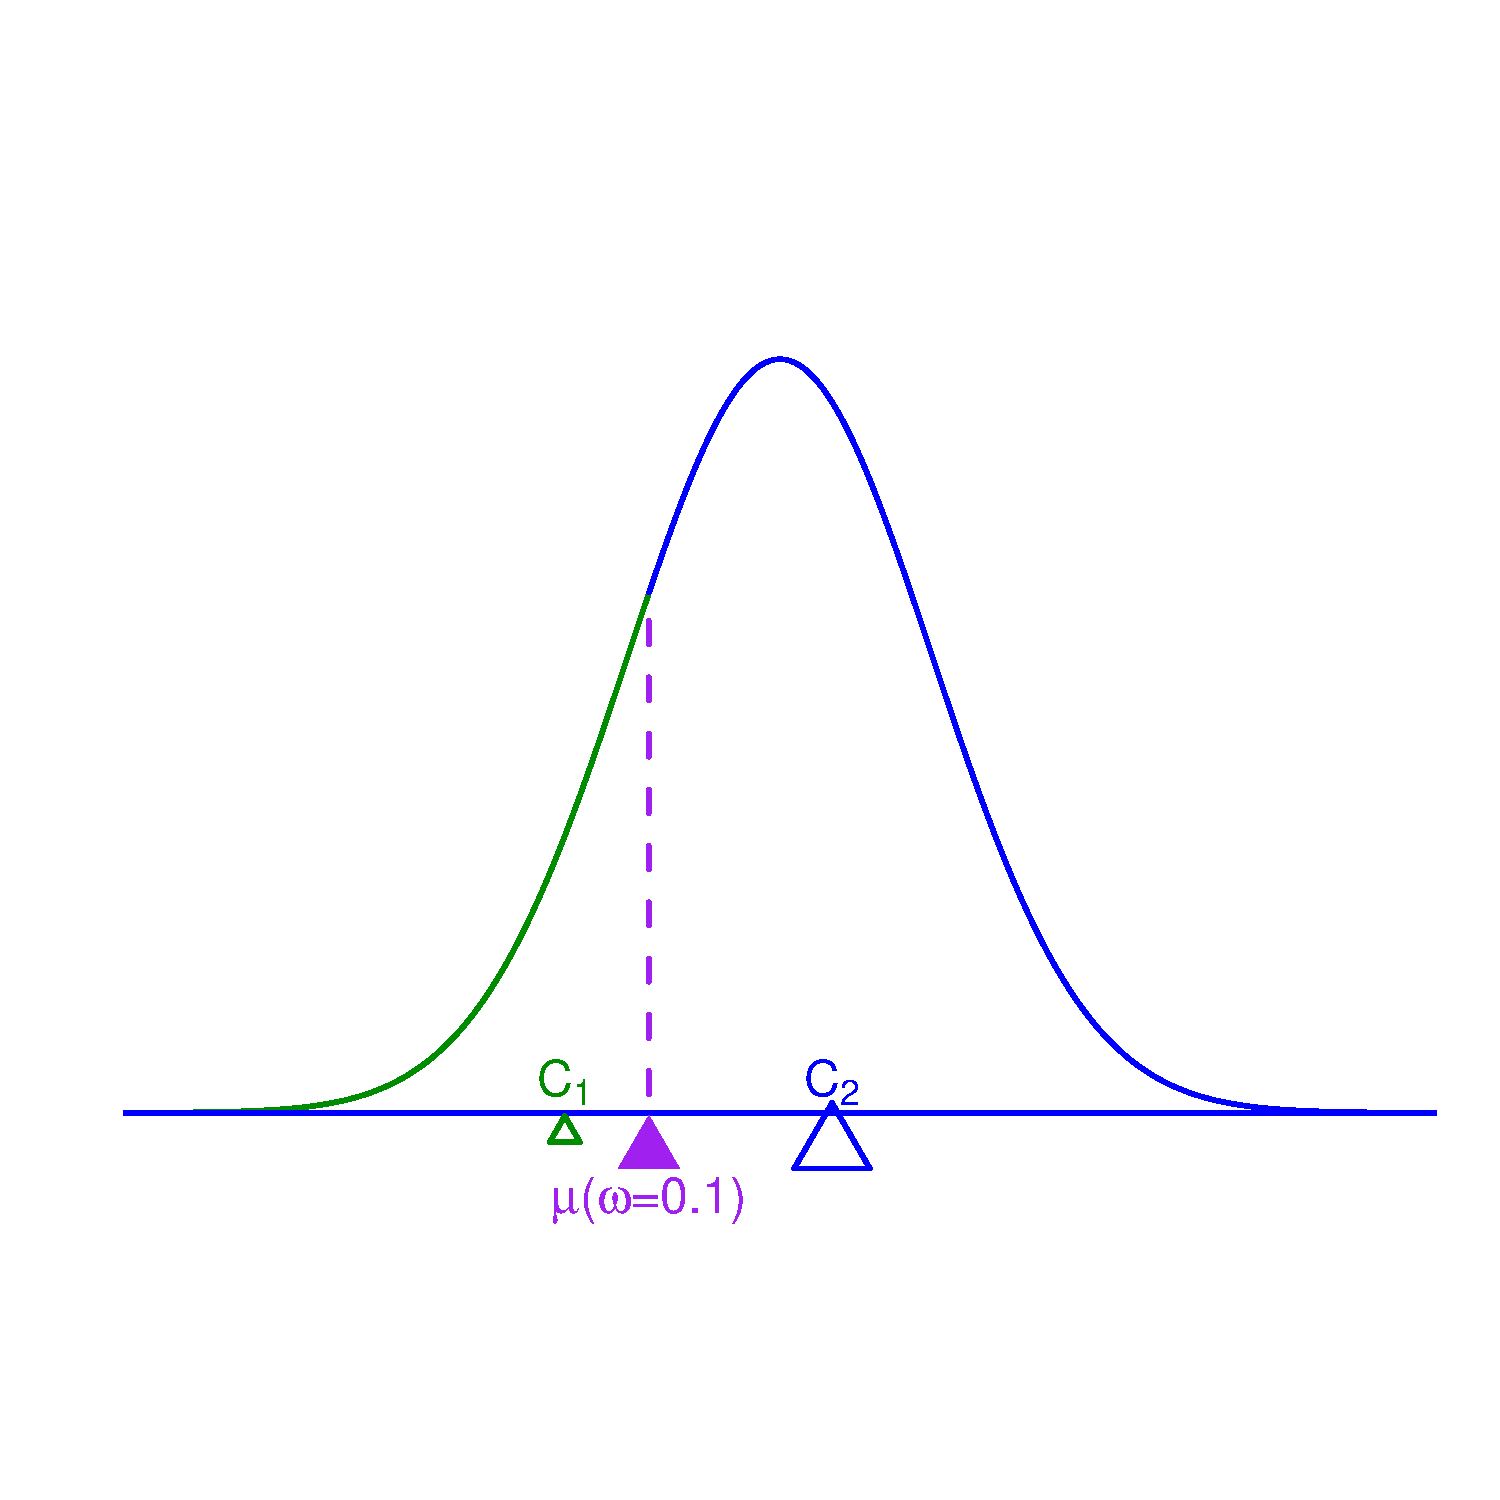
\includegraphics{Assignment3_files/figure-latex/unnamed-chunk-2-1.pdf}
\#\# (b) Modify the plot by choosing nicer colours, etc. in order to
improve it. This should be another plot. {[}2 marks{]}

\begin{Shaded}
\begin{Highlighting}[]
\CommentTok{# sequence for generating Bell graph}
\NormalTok{x <-}\StringTok{ }\KeywordTok{seq}\NormalTok{(}\OperatorTok{-}\DecValTok{4}\NormalTok{, }\DecValTok{4}\NormalTok{, }\DataTypeTok{length =} \DecValTok{1000}\NormalTok{)}

\CommentTok{# line ploting of elements below -0.0862}
\NormalTok{xplot <-}\StringTok{ }\NormalTok{x[x }\OperatorTok{<}\StringTok{ }\OperatorTok{-}\FloatTok{0.862}\NormalTok{]}
\NormalTok{yplot <-}\StringTok{ }\KeywordTok{dnorm}\NormalTok{(xplot, }\DataTypeTok{mean =} \DecValTok{0}\NormalTok{, }\DataTypeTok{sd =} \DecValTok{1}\NormalTok{)}
\KeywordTok{plot}\NormalTok{(xplot, yplot, }\DataTypeTok{type =} \StringTok{"l"}\NormalTok{, }\DataTypeTok{col=}\KeywordTok{rgb}\NormalTok{(}\DecValTok{0}\NormalTok{, }\DecValTok{1}\NormalTok{, }\DecValTok{0}\NormalTok{, .}\DecValTok{3}\NormalTok{), }\DataTypeTok{lwd =} \DecValTok{3}\NormalTok{, }\DataTypeTok{axes =} \OtherTok{FALSE}\NormalTok{, }\DataTypeTok{frame.plot =} \OtherTok{FALSE}\NormalTok{, }\DataTypeTok{ann =} \OtherTok{FALSE}\NormalTok{, }\DataTypeTok{ylim =} \KeywordTok{c}\NormalTok{(}\OperatorTok{-}\NormalTok{.}\DecValTok{1}\NormalTok{, .}\DecValTok{5}\NormalTok{), }\DataTypeTok{xlim =} \KeywordTok{c}\NormalTok{(}\OperatorTok{-}\DecValTok{4}\NormalTok{, }\DecValTok{4}\NormalTok{))}

\CommentTok{# Ploygon filling of area below -0.862}
\NormalTok{m <-}\StringTok{ }\KeywordTok{length}\NormalTok{(xplot)                         }
\NormalTok{x.poly <-}\StringTok{ }\KeywordTok{c}\NormalTok{(xplot, xplot[m], xplot[}\DecValTok{1}\NormalTok{])        }\CommentTok{# Adjoin two x-coordinates}
\NormalTok{y.poly <-}\StringTok{ }\KeywordTok{c}\NormalTok{(yplot, }\DecValTok{0}\NormalTok{, }\DecValTok{0}\NormalTok{)                      }\CommentTok{# .. and the corresponding y-coordinates}
\KeywordTok{polygon}\NormalTok{(x.poly, y.poly, }\DataTypeTok{col=}\KeywordTok{rgb}\NormalTok{(}\DecValTok{0}\NormalTok{, }\DecValTok{1}\NormalTok{, }\DecValTok{0}\NormalTok{, .}\DecValTok{3}\NormalTok{), }\DataTypeTok{border=}\OtherTok{NA}\NormalTok{)}

\CommentTok{# line plotting of elements above or equal to -0.862 }
\NormalTok{xline <-}\StringTok{ }\NormalTok{x[x }\OperatorTok{>=}\StringTok{ }\OperatorTok{-}\FloatTok{0.862}\NormalTok{]}
\NormalTok{yline <-}\StringTok{ }\KeywordTok{dnorm}\NormalTok{(xline, }\DataTypeTok{mean =} \DecValTok{0}\NormalTok{, }\DataTypeTok{sd =} \DecValTok{1}\NormalTok{)}
\KeywordTok{lines}\NormalTok{(}\DataTypeTok{x =}\NormalTok{ xline, }\DataTypeTok{y =}\NormalTok{ yline, }\DataTypeTok{col =} \KeywordTok{rgb}\NormalTok{(}\DecValTok{0}\NormalTok{, }\DecValTok{0}\NormalTok{, }\DecValTok{1}\NormalTok{, .}\DecValTok{3}\NormalTok{), }\DataTypeTok{lwd =} \DecValTok{3}\NormalTok{)}

\CommentTok{# Ploygon filling of elements above or equal to -0.862}
\NormalTok{m <-}\StringTok{ }\KeywordTok{length}\NormalTok{(xline)                         }
\NormalTok{x.poly <-}\StringTok{ }\KeywordTok{c}\NormalTok{(xline, xline[m], xline[}\DecValTok{1}\NormalTok{])        }\CommentTok{# Adjoin two x-coordinates}
\NormalTok{y.poly <-}\StringTok{ }\KeywordTok{c}\NormalTok{(yline, }\DecValTok{0}\NormalTok{, }\DecValTok{0}\NormalTok{)                      }\CommentTok{# .. and the corresponding y-coordinates}
\KeywordTok{polygon}\NormalTok{(x.poly, y.poly, }\DataTypeTok{col=}\KeywordTok{rgb}\NormalTok{(}\DecValTok{0}\NormalTok{, }\DecValTok{0}\NormalTok{, }\DecValTok{1}\NormalTok{, .}\DecValTok{3}\NormalTok{), }\DataTypeTok{border=}\OtherTok{NA}\NormalTok{)}

\CommentTok{# Partitioning line}
\NormalTok{meanOmega <-}\StringTok{ }\KeywordTok{dnorm}\NormalTok{(}\OperatorTok{-}\FloatTok{0.862}\NormalTok{, }\DataTypeTok{mean =} \DecValTok{0}\NormalTok{, }\DataTypeTok{sd =} \DecValTok{1}\NormalTok{)}
\KeywordTok{lines}\NormalTok{(}\DataTypeTok{x =} \KeywordTok{c}\NormalTok{(}\OperatorTok{-}\NormalTok{.}\DecValTok{862}\NormalTok{, }\OperatorTok{-}\NormalTok{.}\DecValTok{862}\NormalTok{), }\DataTypeTok{y =}\KeywordTok{c}\NormalTok{(}\OperatorTok{-}\NormalTok{.}\DecValTok{02}\NormalTok{, meanOmega), }\DataTypeTok{col =} \StringTok{"purple"}\NormalTok{, }\DataTypeTok{lty=}\StringTok{"6666"}\NormalTok{, }\DataTypeTok{lwd =} \DecValTok{3}\NormalTok{)}

\CommentTok{#plotting and text}
\KeywordTok{points}\NormalTok{(}\DataTypeTok{x =} \OperatorTok{-}\NormalTok{.}\DecValTok{862}\NormalTok{, }\DataTypeTok{y =} \OperatorTok{-}\NormalTok{.}\DecValTok{02}\NormalTok{, }\DataTypeTok{pch =} \DecValTok{17}\NormalTok{, }\DataTypeTok{col =} \StringTok{"purple"}\NormalTok{, }\DataTypeTok{cex =} \DecValTok{4}\NormalTok{)}
\KeywordTok{text}\NormalTok{(}\DataTypeTok{x =}  \OperatorTok{-}\NormalTok{.}\DecValTok{862}\NormalTok{, }\DataTypeTok{y =} \OperatorTok{-}\NormalTok{.}\DecValTok{03}\NormalTok{, }\DataTypeTok{labels =} \KeywordTok{expression}\NormalTok{(}\KeywordTok{paste}\NormalTok{(mu, }\StringTok{"("}\NormalTok{, omega,}\StringTok{"="}\NormalTok{, }\StringTok{"0.1)"}\NormalTok{)), }\DataTypeTok{col =} \StringTok{"purple"}\NormalTok{, }\DataTypeTok{pos =} \DecValTok{1}\NormalTok{, }\DataTypeTok{cex=}\DecValTok{2}\NormalTok{)}
\KeywordTok{text}\NormalTok{(}\DataTypeTok{x =}  \OperatorTok{-}\FloatTok{1.415}\NormalTok{, }\DataTypeTok{y =} \OperatorTok{-}\NormalTok{.}\DecValTok{004}\NormalTok{, }\DataTypeTok{labels =} \KeywordTok{expression}\NormalTok{(}\StringTok{'C'}\NormalTok{[}\DecValTok{1}\NormalTok{]), }\DataTypeTok{col =} \StringTok{"white"}\NormalTok{, }\DataTypeTok{pos =} \DecValTok{3}\NormalTok{, }\DataTypeTok{cex=}\DecValTok{4}\NormalTok{)}
\KeywordTok{text}\NormalTok{(}\DataTypeTok{x =}  \FloatTok{0.342}\NormalTok{, }\DataTypeTok{y =} \OperatorTok{-}\NormalTok{.}\DecValTok{004}\NormalTok{, }\DataTypeTok{labels =} \KeywordTok{expression}\NormalTok{(}\StringTok{'C'}\NormalTok{[}\DecValTok{2}\NormalTok{]), }\DataTypeTok{col =} \StringTok{"white"}\NormalTok{, }\DataTypeTok{pos =} \DecValTok{3}\NormalTok{, }\DataTypeTok{cex=}\DecValTok{4}\NormalTok{)}
\end{Highlighting}
\end{Shaded}

\begin{figure}
\centering
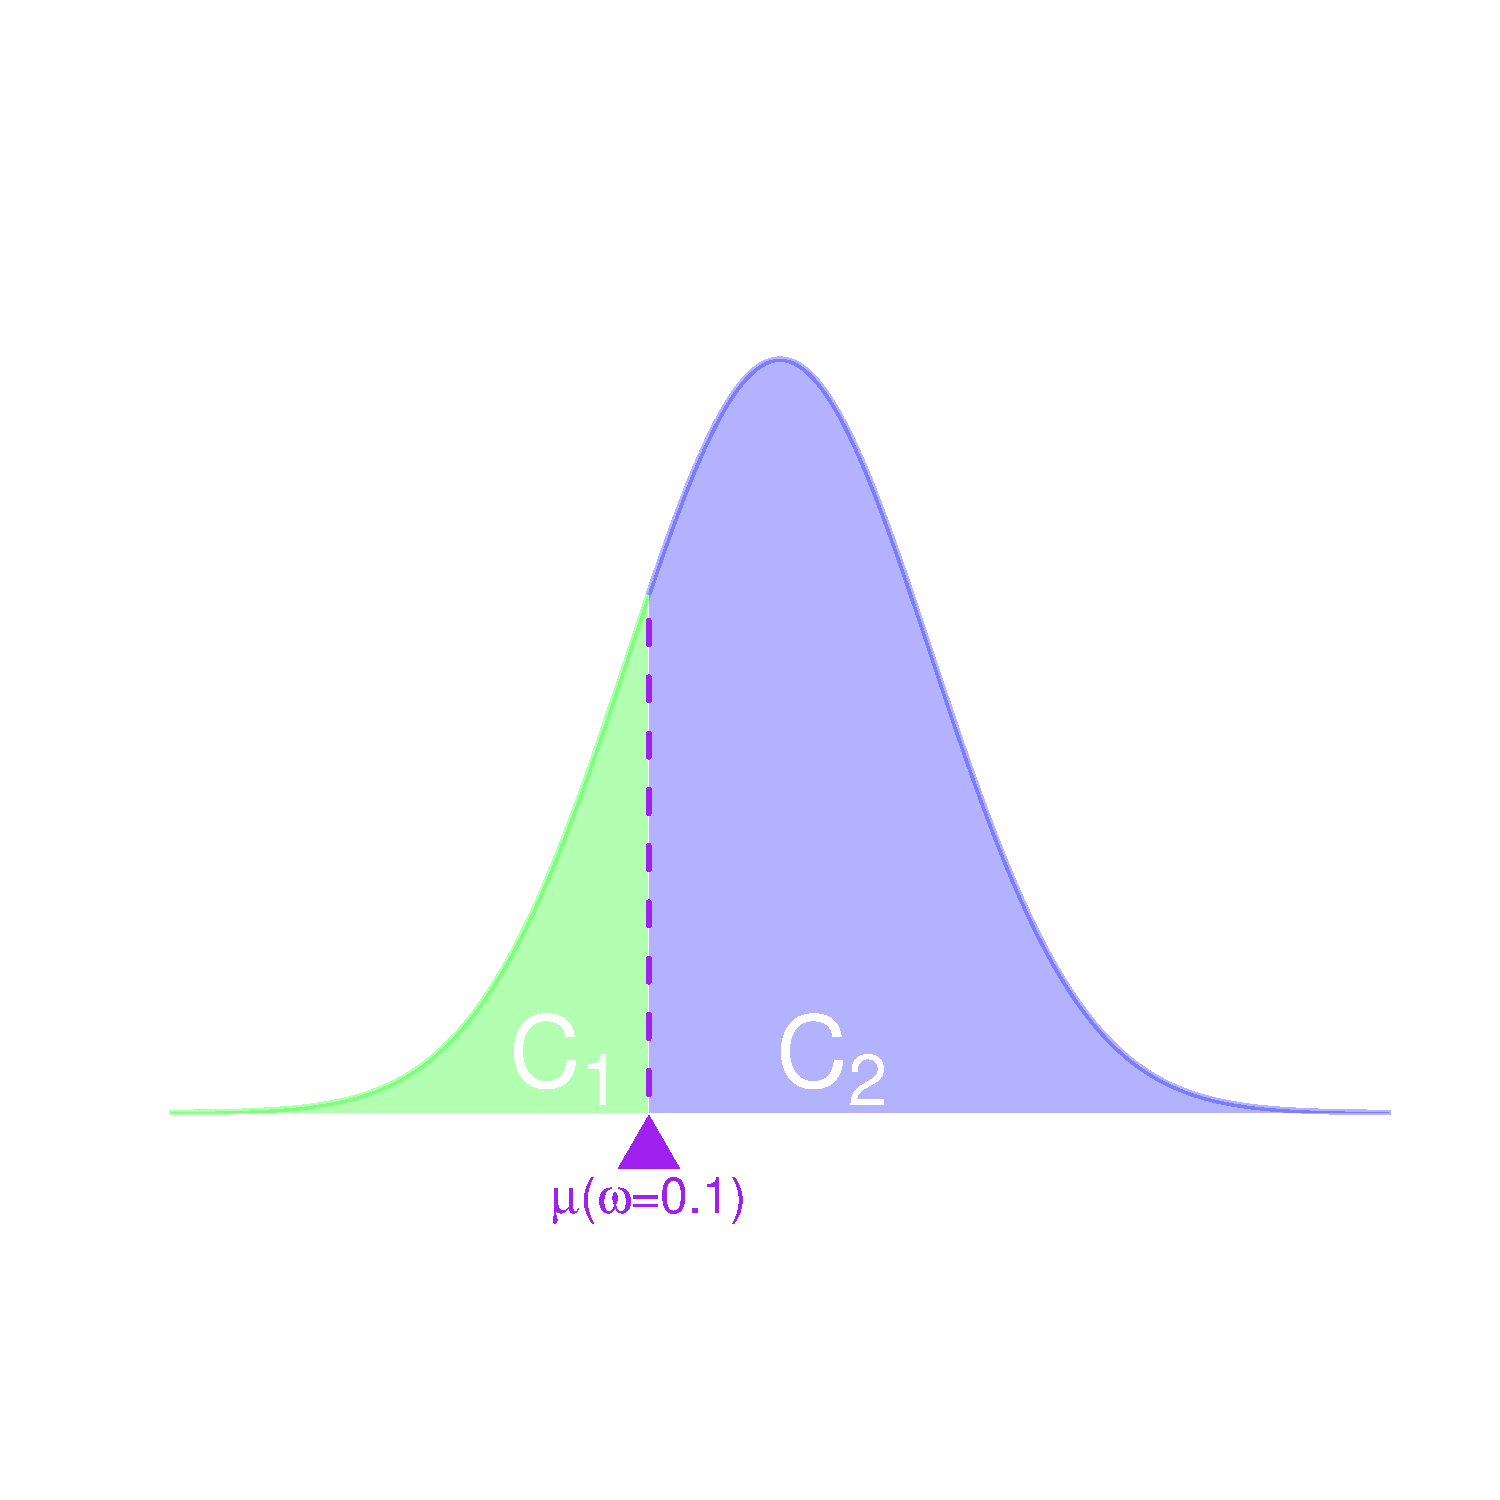
\includegraphics{Assignment3_files/figure-latex/unnamed-chunk-3-1.pdf}
\caption{Figure 2: Illustration of the interpretation of expectiles in
terms of centres of balance: the hollow triangles at positions c1 and
c2. Here, the vertical dashed line is at the 0.1-expectile, and the
solid triangle at µ(?? = 0.1).}
\end{figure}

\subsection{Question 3 {[}10 marks{]} Consider Fig. 3. Use R to
reproduce the gure as closely as possible. The outer perimeter is a
circle.}\label{question-3-10-marks-consider-fig.-3.-use-r-to-reproduce-the-gure-as-closely-as-possible.-the-outer-perimeter-is-a-circle.}

\begin{Shaded}
\begin{Highlighting}[]
\KeywordTok{plot.new}\NormalTok{()}
\KeywordTok{plot.window}\NormalTok{(}\DataTypeTok{xlim =} \KeywordTok{c}\NormalTok{(}\OperatorTok{-}\DecValTok{2}\NormalTok{, }\DecValTok{2}\NormalTok{), }\DataTypeTok{ylim =} \KeywordTok{c}\NormalTok{(}\OperatorTok{-}\DecValTok{2}\NormalTok{, }\DecValTok{2}\NormalTok{), }\DataTypeTok{asp =} \DecValTok{1}\NormalTok{)}

\NormalTok{theta0 <-}\StringTok{ }\KeywordTok{seq}\NormalTok{(}\DecValTok{0}\NormalTok{, }\DecValTok{2} \OperatorTok{*}\StringTok{ }\NormalTok{pi, }\DataTypeTok{length =} \DecValTok{150}\NormalTok{)}

\NormalTok{x <-}\StringTok{ }\DecValTok{2} \OperatorTok{*}\StringTok{ }\KeywordTok{cos}\NormalTok{(theta0) }
\NormalTok{y <-}\StringTok{ }\DecValTok{2} \OperatorTok{*}\StringTok{ }\KeywordTok{sin}\NormalTok{(theta0)}

\KeywordTok{polygon}\NormalTok{(x, y, }\DataTypeTok{col =} \StringTok{"darkseagreen"}\NormalTok{ , }\DataTypeTok{border =} \StringTok{"black"}\NormalTok{, }\DataTypeTok{lwd =} \DecValTok{2}\NormalTok{)}

\NormalTok{theta <-}\StringTok{ }\KeywordTok{seq}\NormalTok{(}\DecValTok{0}\NormalTok{, }\DecValTok{6}\OperatorTok{*}\NormalTok{pi, }\DataTypeTok{length =} \DecValTok{150}\NormalTok{)}

\CommentTok{# four curves in circle}
\NormalTok{spiralCurve <-}\StringTok{ }\DecValTok{1}\OperatorTok{/}\NormalTok{(}\DecValTok{3}\OperatorTok{*}\NormalTok{pi)}

\NormalTok{r1 <-}\StringTok{ }\NormalTok{spiralCurve }\OperatorTok{*}\StringTok{ }\NormalTok{theta}
\NormalTok{r2 <-}\StringTok{ }\NormalTok{(spiralCurve }\OperatorTok{+}\StringTok{ }\NormalTok{.}\DecValTok{021}\NormalTok{) }\OperatorTok{*}\StringTok{ }\NormalTok{theta}

\NormalTok{x1 <-}\StringTok{ }\NormalTok{r1 }\OperatorTok{*}\StringTok{ }\KeywordTok{cos}\NormalTok{(theta) }
\NormalTok{y1 <-}\StringTok{ }\NormalTok{r1 }\OperatorTok{*}\StringTok{ }\KeywordTok{sin}\NormalTok{(theta)}

\NormalTok{x2 <-}\StringTok{ }\NormalTok{r2 }\OperatorTok{*}\StringTok{ }\KeywordTok{cos}\NormalTok{(theta)}
\NormalTok{y2 <-}\StringTok{ }\NormalTok{r2 }\OperatorTok{*}\StringTok{ }\KeywordTok{sin}\NormalTok{(theta)}

\CommentTok{# verification of distance that should not exceed 2 units}
\ControlFlowTok{for}\NormalTok{ (i }\ControlFlowTok{in} \DecValTok{1}\OperatorTok{:}\DecValTok{150}\NormalTok{) \{}
  \ControlFlowTok{if}\NormalTok{(}\KeywordTok{sqrt}\NormalTok{((x2[i]}\OperatorTok{^}\DecValTok{2}\NormalTok{) }\OperatorTok{+}\StringTok{ }\NormalTok{(y2[i]}\OperatorTok{^}\DecValTok{2}\NormalTok{)) }\OperatorTok{>}\StringTok{ }\DecValTok{2}\NormalTok{) \{}
\NormalTok{    x2[i] <-}\StringTok{ }\DecValTok{2} \OperatorTok{*}\StringTok{ }\KeywordTok{cos}\NormalTok{(theta[i])}
\NormalTok{    y2[i] <-}\StringTok{ }\DecValTok{2} \OperatorTok{*}\StringTok{ }\KeywordTok{sin}\NormalTok{(theta[i])}
\NormalTok{  \}}
\NormalTok{\}}

\KeywordTok{lines}\NormalTok{(x1, y1, }\DataTypeTok{col =} \StringTok{"red"}\NormalTok{, }\DataTypeTok{type =} \StringTok{'l'}\NormalTok{)}
\KeywordTok{lines}\NormalTok{(x2, y2, }\DataTypeTok{col =} \StringTok{"red"}\NormalTok{, }\DataTypeTok{type =} \StringTok{'l'}\NormalTok{)}

\KeywordTok{polygon}\NormalTok{(}\KeywordTok{c}\NormalTok{(x1, }\KeywordTok{rev}\NormalTok{(x2)), }\KeywordTok{c}\NormalTok{(y1, }\KeywordTok{rev}\NormalTok{(y2)), }\DataTypeTok{col =} \StringTok{"white"}\NormalTok{, }\DataTypeTok{border =} \StringTok{"red"}\NormalTok{, }\DataTypeTok{lwd =} \DecValTok{4}\NormalTok{)}
\end{Highlighting}
\end{Shaded}


\includegraphics{Assignment3_files/figure-latex/unnamed-chunk-4-1.pdf}
\#\#Question 4. {[}24 marks{]} Consider Fig. 4, which displays a BBC
News graphic obtained from an article on recent Australian heatwaves.
\#\#\#(a) The data from which the plot was made was unavailable from the
BBC website. Instead, I downloaded something very similar from
\url{http://www.bom.gov.au/} and it is available to you. The data
happens to come from Sydney (pronounced Seedney). Hence your plot won't
be exactly the same data-wise, nevertheless you can reproduce it
otherwise the same. Read the data into R. Then check the annual means
column by computing the means over all months-you are checking the
integrity of the data. Comment. {[}5 marks{]}

\begin{Shaded}
\begin{Highlighting}[]
\NormalTok{bbcData <-}\StringTok{ }\KeywordTok{read.csv}\NormalTok{(}\StringTok{'IDCJAC0002-066062-Data12edited.csv'}\NormalTok{)}

\NormalTok{bbcData}\OperatorTok{$}\NormalTok{ComputedMean <-}\StringTok{ }\KeywordTok{round}\NormalTok{(}\KeywordTok{rowMeans}\NormalTok{(bbcData[,}\DecValTok{4}\OperatorTok{:}\DecValTok{16}\NormalTok{], }\DataTypeTok{na.rm =} \OtherTok{TRUE}\NormalTok{), }\DecValTok{2}\NormalTok{)}

\NormalTok{result <-}\StringTok{ }\KeywordTok{any}\NormalTok{(bbcData}\OperatorTok{$}\NormalTok{ComputedMean }\OperatorTok{!=}\StringTok{ }\NormalTok{bbcData}\OperatorTok{$}\NormalTok{Annual)}
\ControlFlowTok{if}\NormalTok{(}\KeywordTok{is.na}\NormalTok{(result)) \{}
  \StringTok{'Some values are Not Available.'}
\NormalTok{\} }\ControlFlowTok{else} \ControlFlowTok{if}\NormalTok{ (result) \{}
  \StringTok{'Data has Integrity Issue'}
\NormalTok{\} }\ControlFlowTok{else}\NormalTok{ \{}
  \StringTok{'No problem with data.'}
\NormalTok{\}}
\end{Highlighting}
\end{Shaded}

\begin{verbatim}
## [1] "Data has Integrity Issue"
\end{verbatim}

\subsubsection{(b) Try to mimic the figure in R as closely as possible,
except for the BBC logo at the bottom and that the data doesn't match
exactly. {[}10
marks{]}}\label{b-try-to-mimic-the-figure-in-r-as-closely-as-possible-except-for-the-bbc-logo-at-the-bottom-and-that-the-data-doesnt-match-exactly.-10-marks}

\begin{Shaded}
\begin{Highlighting}[]
\NormalTok{bbcData}\OperatorTok{$}\NormalTok{meandiff <-}\StringTok{ }\KeywordTok{round}\NormalTok{(bbcData}\OperatorTok{$}\NormalTok{ComputedMean }\OperatorTok{-}\StringTok{ }\KeywordTok{mean}\NormalTok{(bbcData}\OperatorTok{$}\NormalTok{ComputedMean), }\DecValTok{2}\NormalTok{)}
\end{Highlighting}
\end{Shaded}

\begin{Shaded}
\begin{Highlighting}[]
\NormalTok{bbcData}\OperatorTok{$}\NormalTok{color <-}\StringTok{ }\KeywordTok{ifelse}\NormalTok{(bbcData}\OperatorTok{$}\NormalTok{meandiff }\OperatorTok{>}\StringTok{ }\DecValTok{0}\NormalTok{, }\DecValTok{1}\NormalTok{, }\DecValTok{0}\NormalTok{)}
\NormalTok{bbcData}\OperatorTok{$}\NormalTok{positive <-}\StringTok{ }\KeywordTok{ifelse}\NormalTok{(bbcData}\OperatorTok{$}\NormalTok{meandiff }\OperatorTok{>}\StringTok{ }\DecValTok{0}\NormalTok{, bbcData}\OperatorTok{$}\NormalTok{meandiff, }\DecValTok{0}\NormalTok{)}
\NormalTok{bbcData}\OperatorTok{$}\NormalTok{negitive <-}\StringTok{ }\KeywordTok{ifelse}\NormalTok{(bbcData}\OperatorTok{$}\NormalTok{meandiff }\OperatorTok{<}\StringTok{ }\DecValTok{0}\NormalTok{, bbcData}\OperatorTok{$}\NormalTok{meandiff, }\DecValTok{0}\NormalTok{)}

\NormalTok{mat <-}\StringTok{ }\KeywordTok{matrix}\NormalTok{(bbcData}\OperatorTok{$}\NormalTok{positive, }\DataTypeTok{nrow =} \DecValTok{1}\NormalTok{, }\DataTypeTok{dimnames =} \KeywordTok{list}\NormalTok{(}\KeywordTok{c}\NormalTok{(), bbcData}\OperatorTok{$}\NormalTok{Year))}
\NormalTok{mat <-}\StringTok{ }\KeywordTok{rbind}\NormalTok{(mat, bbcData}\OperatorTok{$}\NormalTok{negitive)}


\KeywordTok{barplot}\NormalTok{(}
  \DataTypeTok{height =}\NormalTok{ mat,}
  \DataTypeTok{col =} \KeywordTok{c}\NormalTok{(}\StringTok{'#cd1c1b'}\NormalTok{,}\StringTok{'#1280a1'}\NormalTok{),}
  \DataTypeTok{las =} \DecValTok{1}\NormalTok{,}
  \DataTypeTok{border =} \OtherTok{NA}\NormalTok{, }
  \DataTypeTok{names.arg =} \KeywordTok{colnames}\NormalTok{(mat),}
  \DataTypeTok{ylim =} \KeywordTok{c}\NormalTok{(}\OperatorTok{-}\DecValTok{8}\NormalTok{, }\DecValTok{8}\NormalTok{),}
  \DataTypeTok{main =} \StringTok{"Australia has been getting warmer"}\NormalTok{,}
  \CommentTok{#mtext = "",}
  \DataTypeTok{sub =} \StringTok{"Note: Average is calculated from 1961-1990 data"}\NormalTok{,}
  \DataTypeTok{adj =} \DecValTok{0}\NormalTok{,}
  \DataTypeTok{cex.main =} \DecValTok{3}\NormalTok{,}
  \DataTypeTok{cex.names =} \FloatTok{2.5}\NormalTok{,}
  \DataTypeTok{cex.axis =} \FloatTok{2.5}\NormalTok{,}
  \DataTypeTok{yaxp =} \KeywordTok{c}\NormalTok{(}\DecValTok{8}\NormalTok{, }\OperatorTok{-}\DecValTok{8}\NormalTok{, }\DecValTok{4}\NormalTok{),}
  \DataTypeTok{ann =} \OtherTok{FALSE}
\NormalTok{)}
\end{Highlighting}
\end{Shaded}

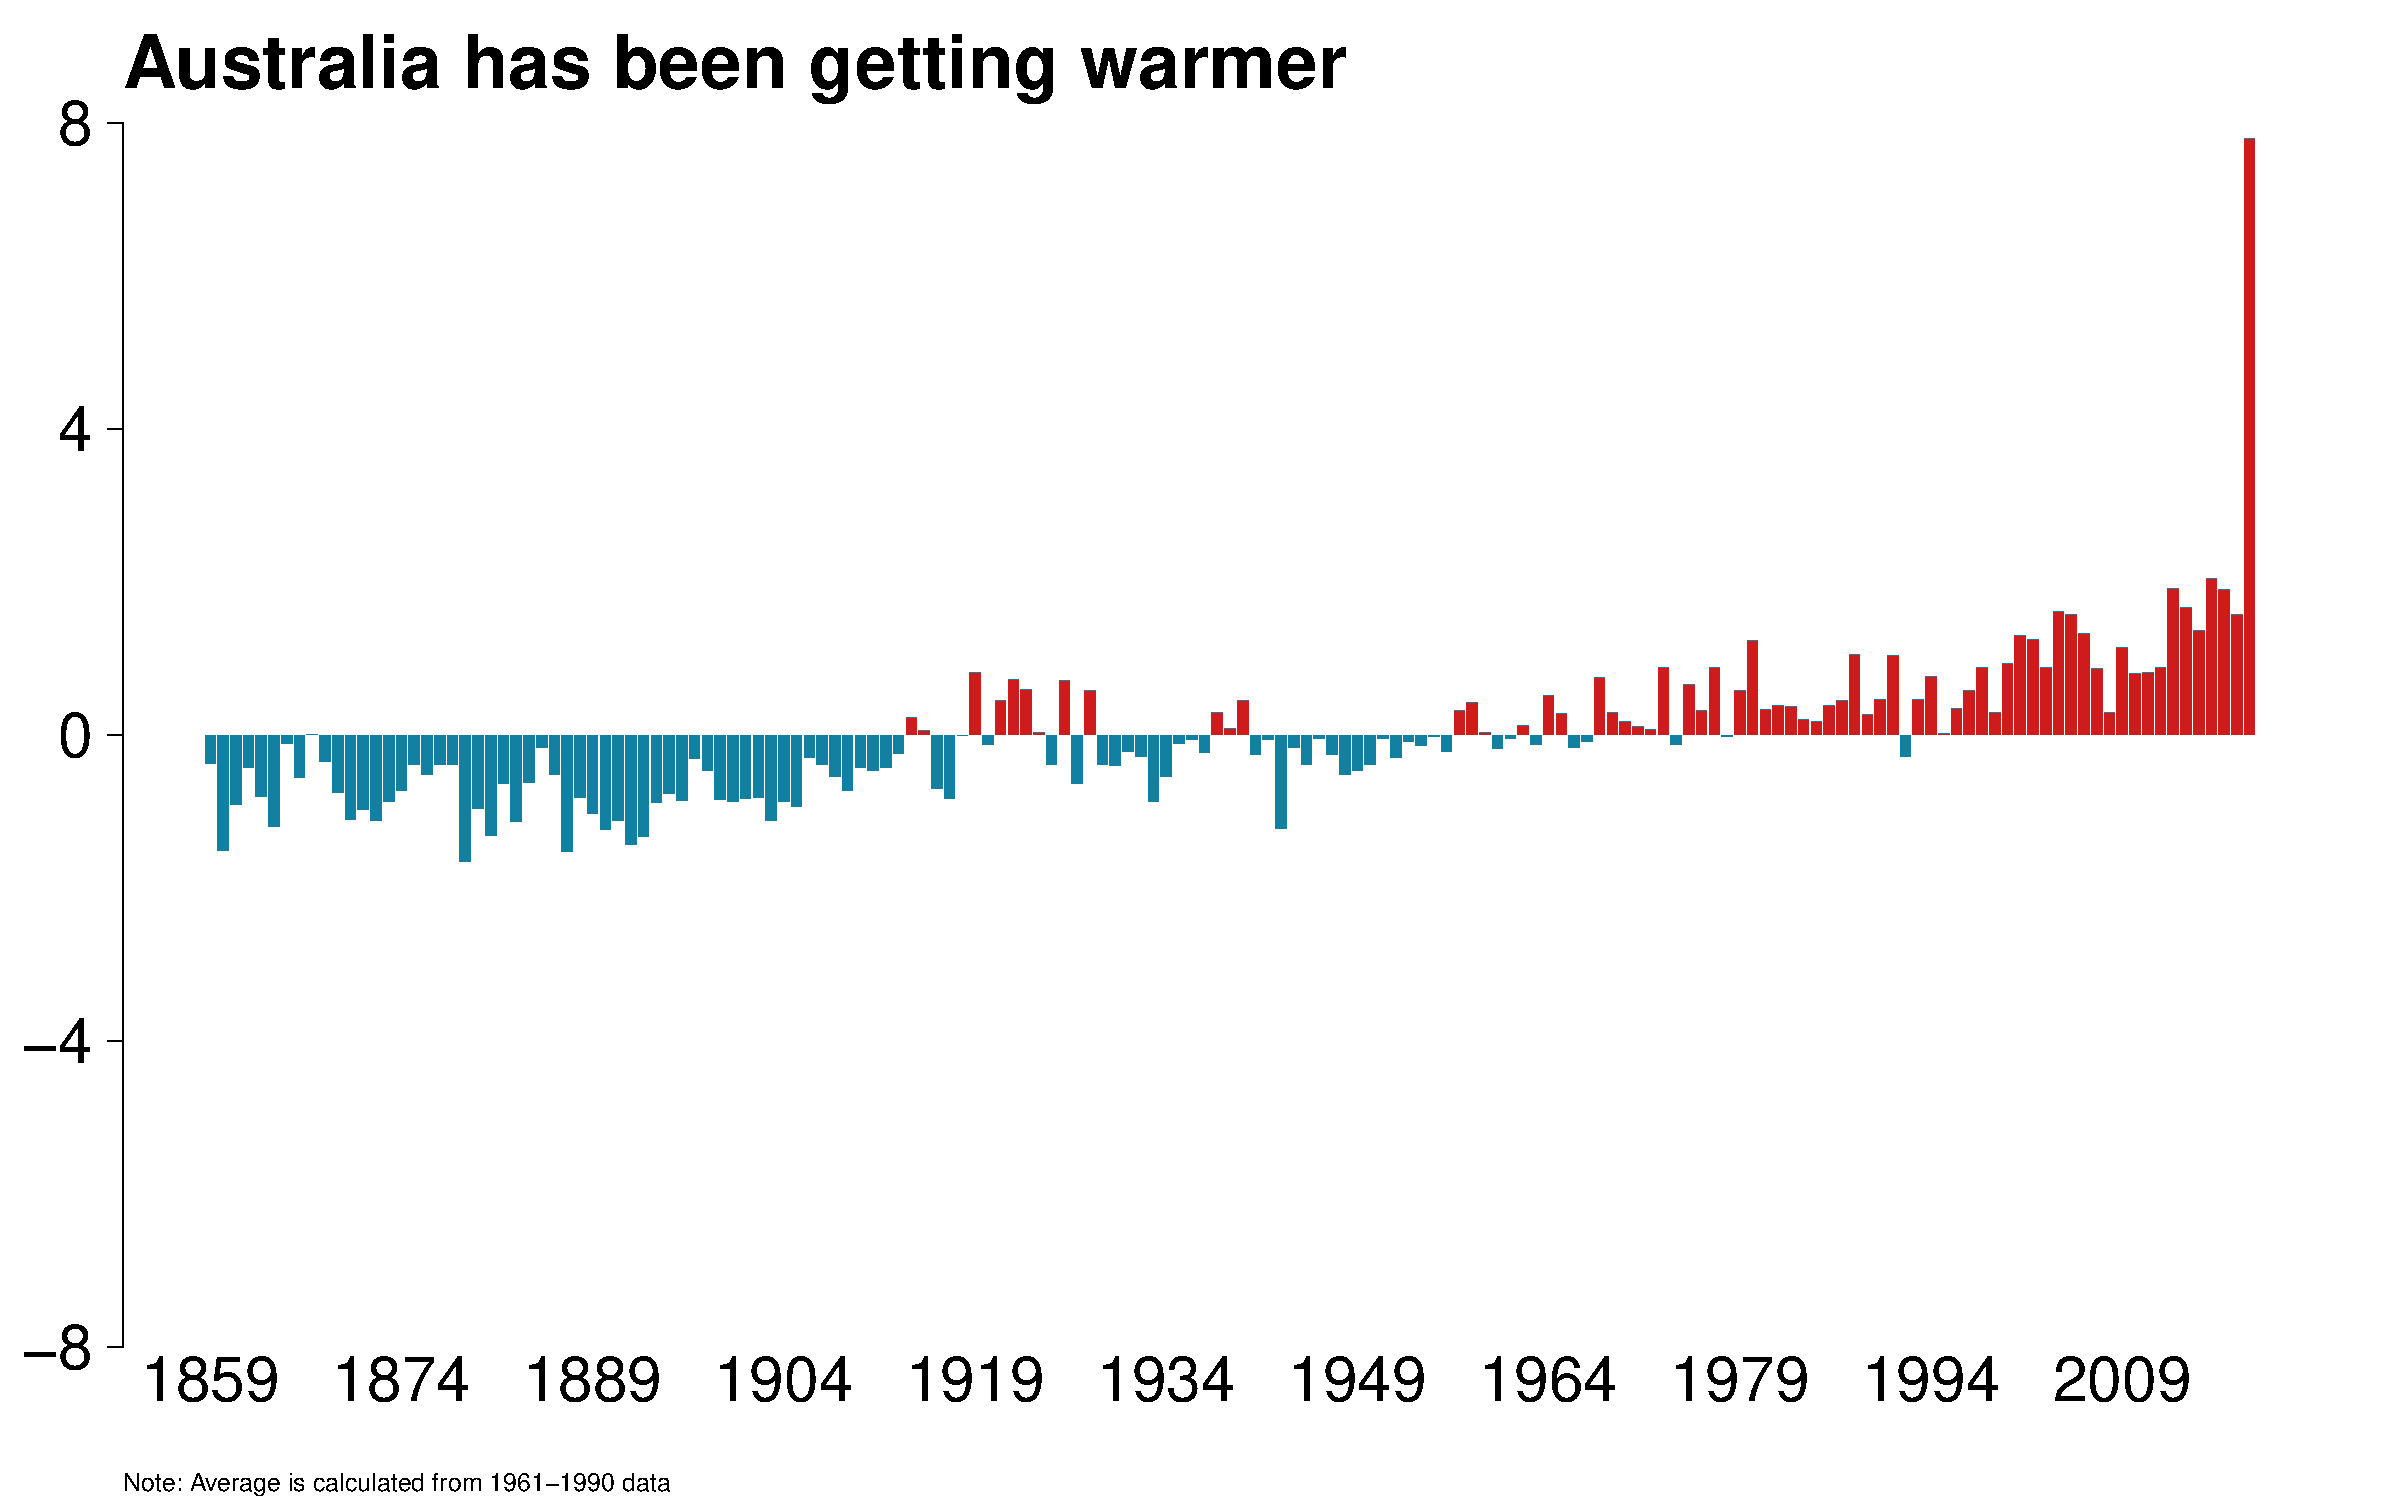
\includegraphics{Assignment3_files/figure-latex/unnamed-chunk-7-1.pdf}

\subsubsection{(c) Add in all years' data and obtain a similar plot, and
use the same centring mean as in (b). Write a paragraph or two
interpreting the plot, i.e., as a statistician, what do we learn from
this plot? {[}5
marks{]}}\label{c-add-in-all-years-data-and-obtain-a-similar-plot-and-use-the-same-centring-mean-as-in-b.-write-a-paragraph-or-two-interpreting-the-plot-i.e.-as-a-statistician-what-do-we-learn-from-this-plot-5-marks}

\begin{Shaded}
\begin{Highlighting}[]
\NormalTok{bbcData}\OperatorTok{$}\NormalTok{total <-}\StringTok{ }\KeywordTok{round}\NormalTok{(}\KeywordTok{rowSums}\NormalTok{(bbcData[,}\DecValTok{4}\OperatorTok{:}\DecValTok{16}\NormalTok{], }\DataTypeTok{na.rm =} \OtherTok{TRUE}\NormalTok{), }\DecValTok{2}\NormalTok{)}

\NormalTok{bbcData}\OperatorTok{$}\NormalTok{positive <-}\StringTok{ }\KeywordTok{ifelse}\NormalTok{(bbcData}\OperatorTok{$}\NormalTok{ComputedMean }\OperatorTok{>}\StringTok{ }\KeywordTok{mean}\NormalTok{(bbcData}\OperatorTok{$}\NormalTok{ComputedMean), bbcData}\OperatorTok{$}\NormalTok{ComputedMean, }\DecValTok{0}\NormalTok{)}
\NormalTok{bbcData}\OperatorTok{$}\NormalTok{negitive <-}\StringTok{ }\KeywordTok{ifelse}\NormalTok{(bbcData}\OperatorTok{$}\NormalTok{ComputedMean }\OperatorTok{<}\StringTok{ }\KeywordTok{mean}\NormalTok{(bbcData}\OperatorTok{$}\NormalTok{ComputedMean), bbcData}\OperatorTok{$}\NormalTok{ComputedMean, }\DecValTok{0}\NormalTok{)}

\NormalTok{mat <-}\StringTok{ }\KeywordTok{matrix}\NormalTok{(bbcData}\OperatorTok{$}\NormalTok{positive, }\DataTypeTok{nrow =} \DecValTok{1}\NormalTok{, }\DataTypeTok{dimnames =} \KeywordTok{list}\NormalTok{(}\KeywordTok{c}\NormalTok{(), bbcData}\OperatorTok{$}\NormalTok{Year))}
\NormalTok{mat <-}\StringTok{ }\KeywordTok{rbind}\NormalTok{(mat, bbcData}\OperatorTok{$}\NormalTok{negitive)}


\KeywordTok{barplot}\NormalTok{(}
  \DataTypeTok{height =}\NormalTok{ mat,}
  \DataTypeTok{col =} \KeywordTok{c}\NormalTok{(}\StringTok{'#cd1c1b'}\NormalTok{,}\StringTok{'#1280a1'}\NormalTok{),}
  \DataTypeTok{las =} \DecValTok{1}\NormalTok{,}
  \DataTypeTok{border =} \OtherTok{NA}\NormalTok{, }
  \DataTypeTok{names.arg =} \KeywordTok{colnames}\NormalTok{(mat),}
  \CommentTok{#ylim = c(-8, 8),}
  \DataTypeTok{main =} \StringTok{"Australia has been getting warmer"}\NormalTok{,}
  \CommentTok{#mtext = "",}
  \DataTypeTok{sub =} \StringTok{"Note: Average is calculated from 1961-1990 data"}\NormalTok{,}
  \DataTypeTok{adj =} \DecValTok{0}\NormalTok{,}
  \DataTypeTok{cex.main =} \DecValTok{3}\NormalTok{,}
  \DataTypeTok{cex.names =} \FloatTok{2.5}\NormalTok{,}
  \DataTypeTok{cex.axis =} \FloatTok{2.5}\NormalTok{,}
  \CommentTok{#yaxp = c(8, -8, 4),}
  \DataTypeTok{ann =} \OtherTok{FALSE}
\NormalTok{)}
\end{Highlighting}
\end{Shaded}

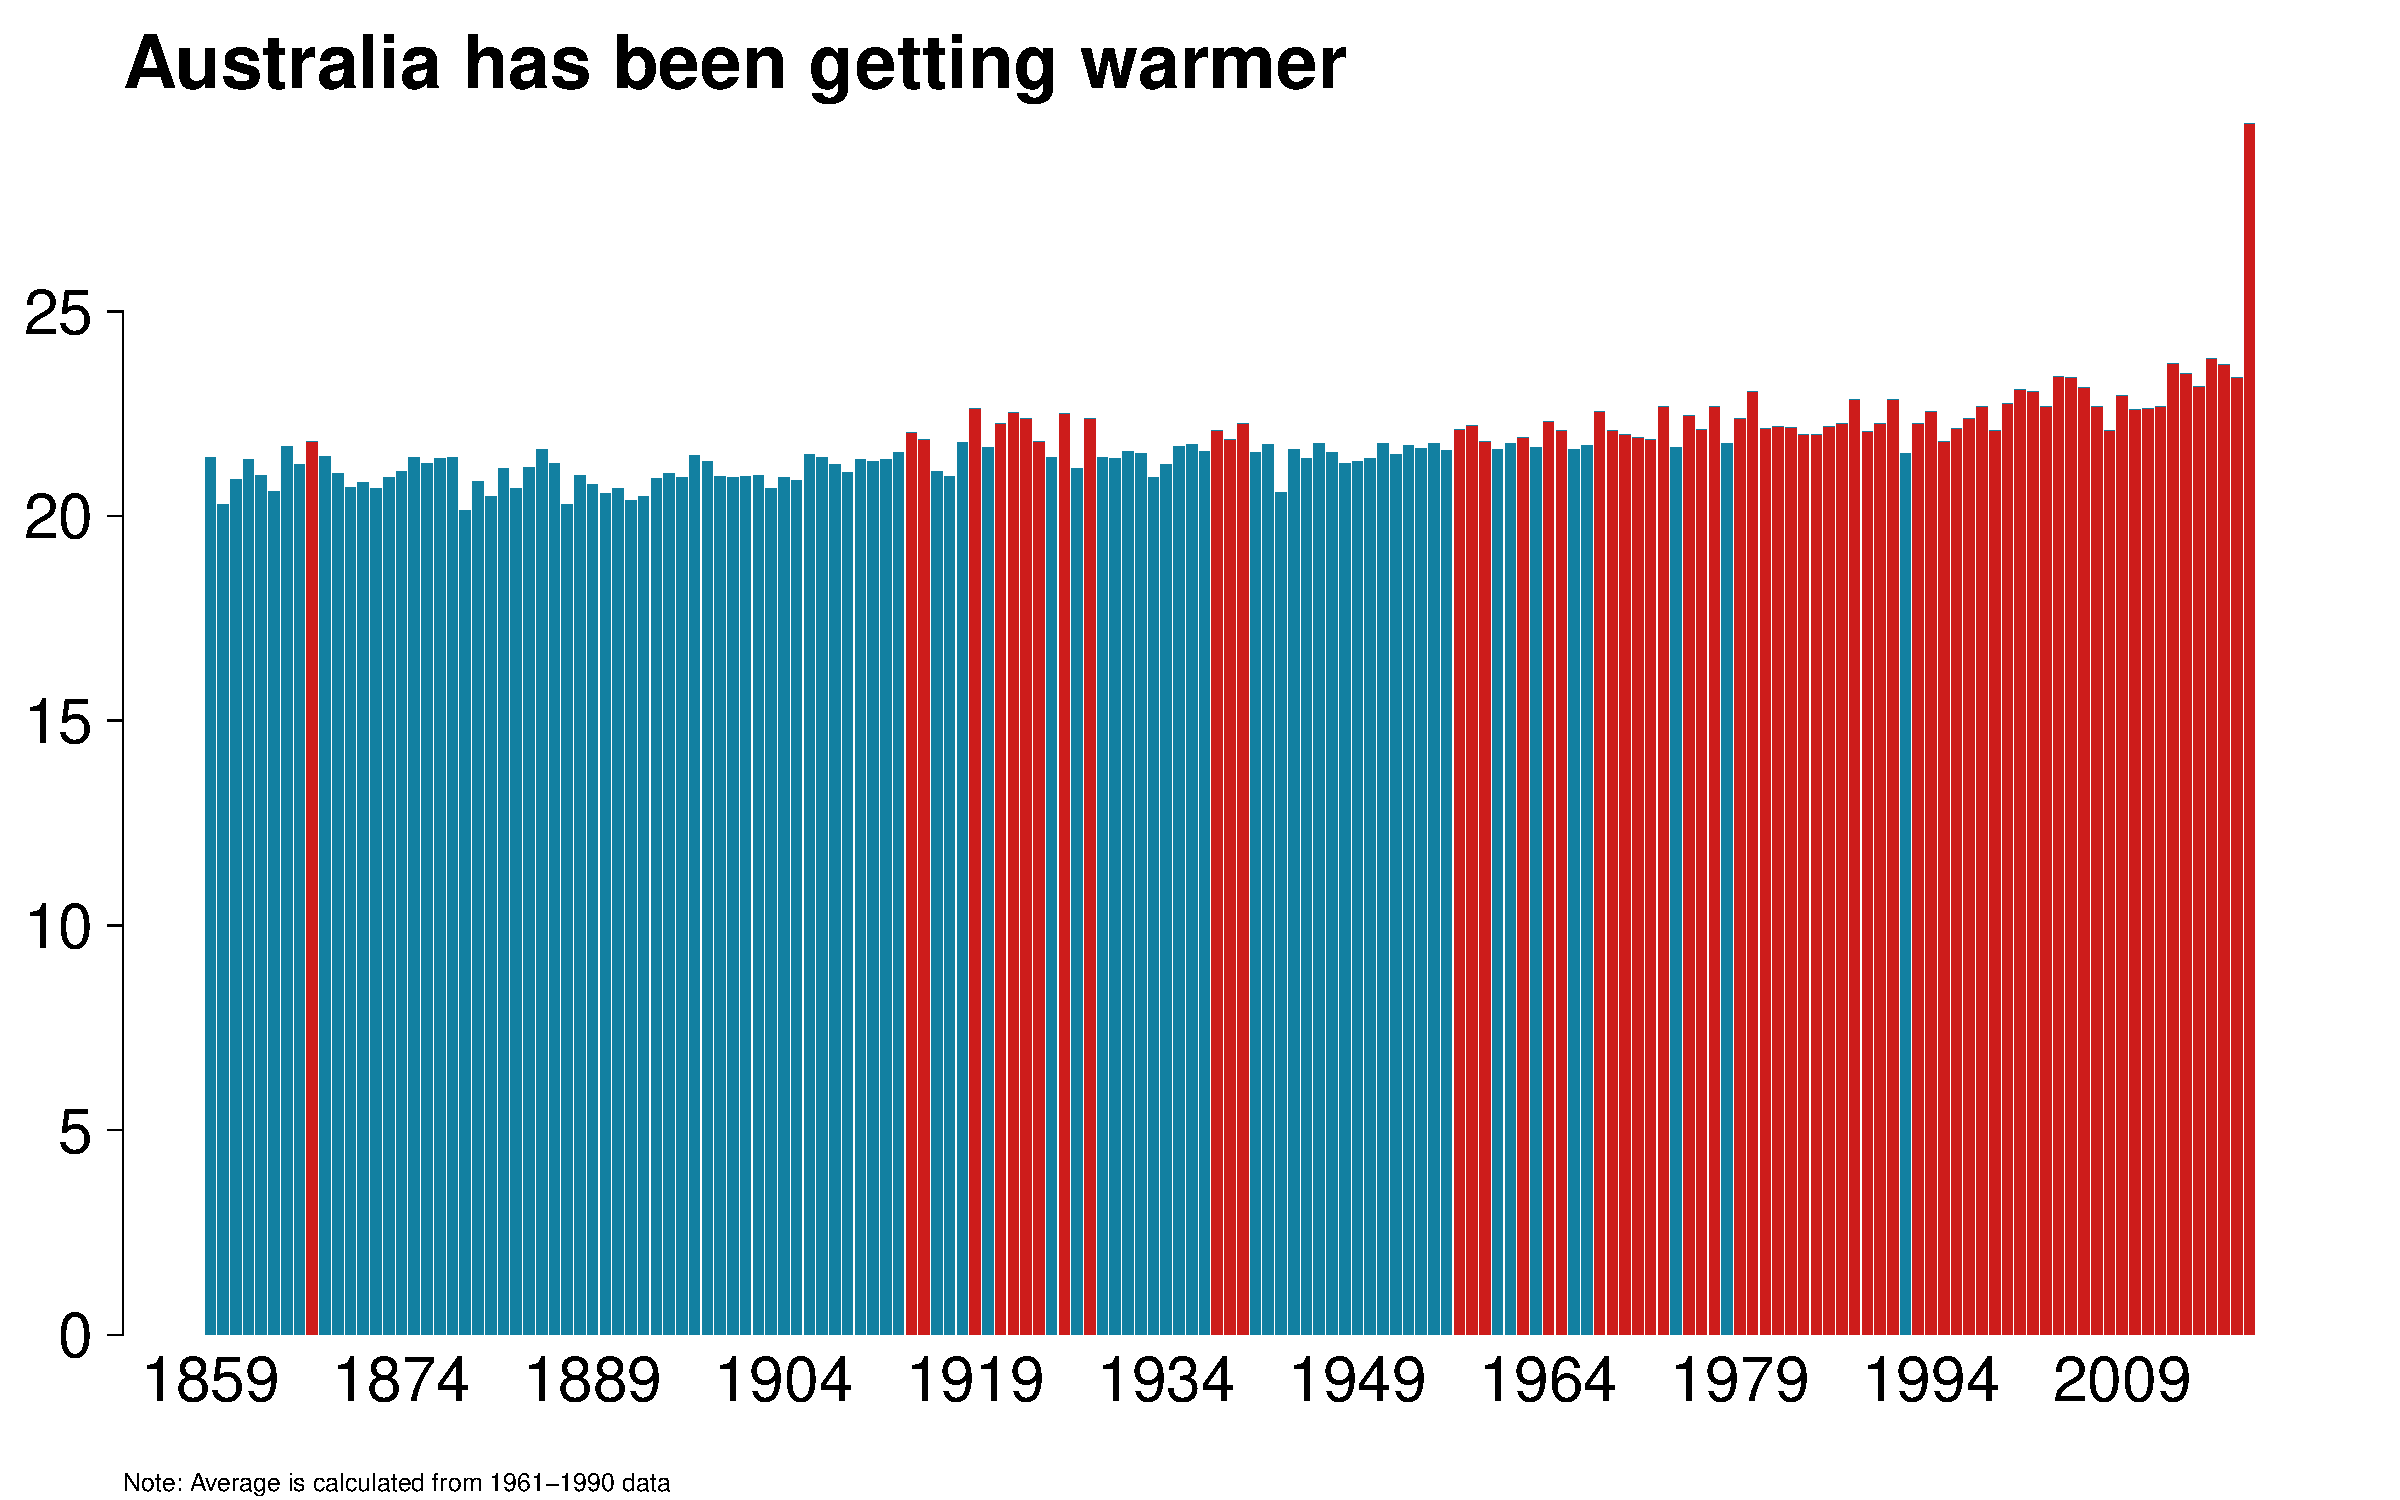
\includegraphics{Assignment3_files/figure-latex/unnamed-chunk-8-1.pdf}

\subsubsection{(d) Predict the annual mean temperature value in the year
2030, and try give a 95\% prediction interval for this. Justify your
method. {[}4
marks{]}}\label{d-predict-the-annual-mean-temperature-value-in-the-year-2030-and-try-give-a-95-prediction-interval-for-this.-justify-your-method.-4-marks}

\begin{Shaded}
\begin{Highlighting}[]
\NormalTok{model <-}\StringTok{ }\KeywordTok{lm}\NormalTok{(ComputedMean}\OperatorTok{~}\NormalTok{Year, }\DataTypeTok{data =}\NormalTok{ bbcData)}

\KeywordTok{predict}\NormalTok{(model, }\KeywordTok{data.frame}\NormalTok{(}\DataTypeTok{Year =} \DecValTok{2030}\NormalTok{), }\DataTypeTok{interval=}\StringTok{"prediction"}\NormalTok{)}
\end{Highlighting}
\end{Shaded}

\begin{verbatim}
##        fit     lwr      upr
## 1 23.16196 21.7637 24.56021
\end{verbatim}

\begin{Shaded}
\begin{Highlighting}[]
\StringTok{'Fitted Model is 23.16196, lower limit is 21.7637 and upper limit is 24.56021'}
\end{Highlighting}
\end{Shaded}

\begin{verbatim}
## [1] "Fitted Model is 23.16196, lower limit is 21.7637 and upper limit is 24.56021"
\end{verbatim}

\subsubsection{(e) Bonus. Suppose in Fig. 4 that temperatures stabilized
beyond the year 2100 and the annual mean temperature above the average
is exponentially distributed with unit mean independently each year.
About how many years after 2100 would somebody have to wait for so that
the probability of experiencing an annual maximum greater than 6.5???C
above the average is at least 5\%? {[}3
marks{]}}\label{e-bonus.-suppose-in-fig.-4-that-temperatures-stabilized-beyond-the-year-2100-and-the-annual-mean-temperature-above-the-average-is-exponentially-distributed-with-unit-mean-independently-each-year.-about-how-many-years-after-2100-would-somebody-have-to-wait-for-so-that-the-probability-of-experiencing-an-annual-maximum-greater-than-6.5c-above-the-average-is-at-least-5-3-marks}


\end{document}
